\documentclass[12pt]{article}

\usepackage{fullpage}
\usepackage[round]{natbib}
\usepackage{multirow}
\usepackage{booktabs}
\usepackage{graphicx}
\usepackage{float}
\usepackage{array}
\newcolumntype{C}[1]{>{\centering\let\newline\\\arraybackslash\hspace{0pt}}m{#1}}
\graphicspath{ {images/} }

\newcounter{acnum}
\newcommand{\actheacnum}{AC\theacnum}
\newcommand{\acref}[1]{AC\ref{#1}}

\newcounter{ucnum}
\newcommand{\uctheucnum}{UC\theucnum}
\newcommand{\uref}[1]{UC\ref{#1}}

\newcounter{mnum}
\newcommand{\mthemnum}{M\themnum}
\newcommand{\mref}[1]{M\ref{#1}}

\begin{document}

\begin{titlepage}
\font\myfont=cmr12 at 38pt
\title{\myfont\vspace{60mm}Zop Design Documentation} 
\author{Ratna Emani, Cole Blanchard, Akshay Mantha}
\date{\today}
\maketitle

\end{titlepage}
\newpage
\textbf{Revision History}\\
\begin{center}
 \begin{tabular}{|C{3cm}|C{3cm}|C{3cm}|C{3cm}|}
 \hline
 \textbf{Developer} & \textbf{Date} & \textbf{Change} & \textbf{Revision Number}\\
 \hline \hline
 Cole Blanchard & November 06 2015 & Introduction, \newline Anticipated and Unlikely Changes, \newline Connection Between Requirements and Design, \newline Pert Chart, \newline Traceability Matrices & 3\\
 \hline
 Ratna Emani & November 06 2015 & Module Hierarchy,\newline Module Decomposition, \newline Use Hierarchy, \newline Gantt Chart & 2\\
 \hline
 Akshay Mantha & November 04 2015 & MIS, \newline Pert Chart & 1\\
 \hline
 \end{tabular}
\end{center}

\newpage
\tableofcontents
\newpage


\section{Introduction}
This document details the design specifications for the implemented modules in Zop.  This document is to be used to simplify navigation through the program for design and maintenance purposes.  This document complements the System Requirement Specifications and the Test Plan.

\section{Anticipated and Unlikely Changes}\label{SecChange}

\subsection{Anticipated Changes}\label{SecAChange}
\begin{description}
\item[\refstepcounter{acnum} \actheacnum \label{acGUI}:] Add a GUI.
\item[\refstepcounter{acnum} \actheacnum \label{acScore}:] Add a score counter.
\item[\refstepcounter{acnum} \actheacnum \label{acTimer}:] Add a timer.
\item[\refstepcounter{acnum} \actheacnum \label{acMouse}:] Add a mouse listener.
\item[\refstepcounter{acnum} \actheacnum \label{acSelect}:] Change how the tiles are selected in a turn
\item[\refstepcounter{acnum} \actheacnum \label{acKeyboard}:] Eliminate keyboard functionality
\item[\refstepcounter{acnum} \actheacnum \label{acTurn}:] Change the algorithm of how turns are made in the game.
\end{description}

\subsection{Unlikely Changes}
\begin{description}
\item[\refstepcounter{ucnum} \uctheucnum \label{ucHighScore}:] Add a High Scores List.
\item[\refstepcounter{ucnum} \uctheucnum \label{ucButtons}:] Start, restart, play again buttons.
\item[\refstepcounter{ucnum} \uctheucnum \label{ucInput}:] tile data stored differently.
\end{description}


\section{Module Hierarchy} \label{SecMH}

Module Hierarchy provides the guidelines of the module design. Modules are sorted
in a hierarchy decomposed by secrets in Table \ref{TblMH}. The modules referred below are the modules that are being implemented and serve as the 'Leaf-nodes' in the hierarchy tree.

\begin{description}
\item [\refstepcounter{mnum} \mthemnum \label{mHH}:] Hardware-Hiding Module
\item [\refstepcounter{mnum} \mthemnum \label{mMain}:] Main Module
\item [\refstepcounter{mnum} \mthemnum \label{mUI}:] userInput Module
\item [\refstepcounter{mnum} \mthemnum \label{mBoard}:] Board Module
\item [\refstepcounter{mnum} \mthemnum \label{mTile}:] Tile Module
\item [\refstepcounter{mnum} \mthemnum \label{mColor}:] colourMatch Module
\item [\refstepcounter{mnum} \mthemnum \label{mAdj}:] adjacent Module
\item [\refstepcounter{mnum} \mthemnum \label{mRemove}:] removeTile Module
\item [\refstepcounter{mnum} \mthemnum \label{mCol}:] checkColumn Module
\item [\refstepcounter{mnum} \mthemnum \label{mDown}:] moveDown Module
\item [\refstepcounter{mnum} \mthemnum \label{mAdd}:] addTile Module
\end{description}
\begin{table}[h!]
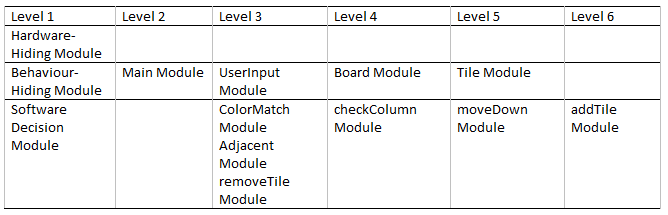
\includegraphics[width = 17cm]{hierTable}
\caption{Modules}
\label{TblRT}
\end{table}

The Operating System (OS) must implement some modules in order to perform other functions. \mref{mHH} is a commonly used to refer to modules that have been implemented by the OS.  Therefore there is no requirement for them to be reimplemented. All the other modules listen below serve to provide an input/output or make logical decisions to implement the rules of Zop.


\section{Connection Between Requirements and Design}
\begin{enumerate}
 \item The product must allow the user to select game pieces.  This requirement is satisfied in the userInput function of the design where the user inputs the coordinates of the piece they want to select.
 \item The product must delete selected pieces of the same colour.  This requirement is implemented with the colourMatch function in the design.
 \item The product must delete selected pieces the are adjacent to each other.  This requirement is met in the adjacent function in the design.
 \item The design fulfils non functional requirements such as security (no password required), cultural, and legal requirements.
 \item Look and feel requirement: zop consists of coloured squares on a grid.  Although we implemented a visual "board" in the console, we have not met this requirement yet.  This is an anticipated change in the future when the GUI is implemented.
 \item Many requirement have not been yet implemented into the design, however these are anticipated changes that will be made in the future.
\end{enumerate}

\section{Module Decomposition}
\subsection{Hardware Hiding Modules (M1)}
\textbf{Secrets:} the primary secret hidden by this module is the hardware/software interfaces. Also the data structures and algorithms used to implement the virtual hardware\\
\textbf{Service:} controls the procedures that are used to handle the hardware/software interface changes with the same general capabilities. This is achieved by using virtual hardware, a digital hardware/software connection it can rely on. \\
\textbf{Implemented By:} OS

\subsection{Main Module (M2)}
\textbf{Secrets:} Hides everything from the game mechanics to the sensitive design decisions.\\
\textbf{Service:} Is used to execute the game, called by the user or the front-end implementation when a GUI is developed.\\
\textbf{Implemented By:} -

\subsection{userInput Module (M3)}
\textbf{Secrets:} Hides all the software decision modules.\\
\textbf{Service:} serves as the only gateway in the behaviour-hiding module to use the software decision modules, reinforcing encapsulation and information hiding. \\
\textbf{Implemented By:} Main Module

\subsection{Board Module (M4)}
\textbf{Secrets:} Hides the Tile object from the rest of the game logic.\\
\textbf{Service:} creates a six index by six index two-dimensional array, and populates the fields with the Tile object.\\
\textbf{Implemented By:} Main Module


\subsection{Tile Module (M5)}
\textbf{Secrets:} generated randomly\\
\textbf{Service:} creates a tile object with a random selection made from a set array of colors. \\
\textbf{Implemented By:} Board Module

\subsection{colorMatch Module (M6)}
\textbf{Secrets:} hides part of the data – Ignores the index location\\
\textbf{Service:} Given a set of Tile objects, the module is responsible for checking the colors of the tile and confirm if they are all same. \\
\textbf{Implemented By:} userInput Module

\subsection{adjacent Module (M7)}
\textbf{Secrets:} hides part of the data – Ignores the index value\\
\textbf{Service:} Given a set of Tile objects, the module is responsible for checking if the tiles are all adjacent to each other – horizontal and/or vertical (not diagonal).\\
\textbf{Implemented By:} userInput Module

\subsection{removeTile Module (M8)}
\textbf{Secrets:} secures the rest of the board tiles to avoid any loss of data\\
\textbf{Service:} Isolates the selected tiles from the remaining pieces to keep track and update the states of the game board. Finally marks the removed tile with a flag.\\
\textbf{Implemented By:} userInput Module

\subsection{checkColumn Module (M9)}
\textbf{Secrets:} secures the order of the rest of the columns on the board to avoid any loss of data\\
\textbf{Service:} Isolates the selected columns and counts the number of flagged tiles and removes them.\\
\textbf{Implemented By:} removeTile Module

\subsection{moveDown Module (M10)}
\textbf{Secrets:} works only with the columns being updated, hiding the rest of the board for being changed\\
\textbf{Service:} with the given column number and the number of missing tiles, moves all the tiles down. Implements the law of gravity within the board.\\
\textbf{Implemented By:} checkColumn Module

\subsection{addTile Module (M11)}
\textbf{Secrets:} accesses only the very top row of the matrix, hiding the rest of the board from being changed\\
\textbf{Service:} with the given column number and the number of missing tiles, addTile fills the missing fields with new Tile objects.\\
\textbf{Implemented By:} moveDown Module

\section{Traceability Matrix} \label{SecTM}

This section shows two traceability matrices: between the modules and the
requirements and between the modules and the anticipated changes.
% the table should use mref, the requirements should be named, use something
% like fref
\subsection{Requirements and modules}
\begin{table}[H]
\centering
\begin{tabular}{p{0.4\textwidth} p{0.6\textwidth}}
\toprule
\textbf{Req.} & \textbf{Modules}\\
\midrule
Select game pieces & \mref{mUI}\\
Display Board & \mref{mBoard}\\
Same Colour Tiles Removed & \mref{mColor}, \mref{mRemove}, M11, M9\\
Adjacent Tiles Removed & \mref{mAdj}, \mref{mRemove}, M11, M9\\
Start Game & \mref{mMain}\\

\bottomrule
\end{tabular}
\caption{Trace Between Requirements and Modules}
\label{TblRT}
\end{table}

\subsection{Anticipated Changes and modules}
\begin{table}[H]
\centering
\begin{tabular}{p{0.4\textwidth} p{0.6\textwidth}}
\toprule
\textbf{AC} & \textbf{Modules}\\
\midrule
AC1 & M4, M5\\
AC2 & M3, M4\\
AC3 & M3, M4\\
AC4 & M4\\
AC5 & M3\\
AC6 & M4\\
AC7 & M4\\
\bottomrule
\end{tabular}
\caption{Trace Between Anticipated Changes and Modules}
\label{TblRT}
\end{table}

\section{Use Hierarchy}
\begin{figure}[h!]
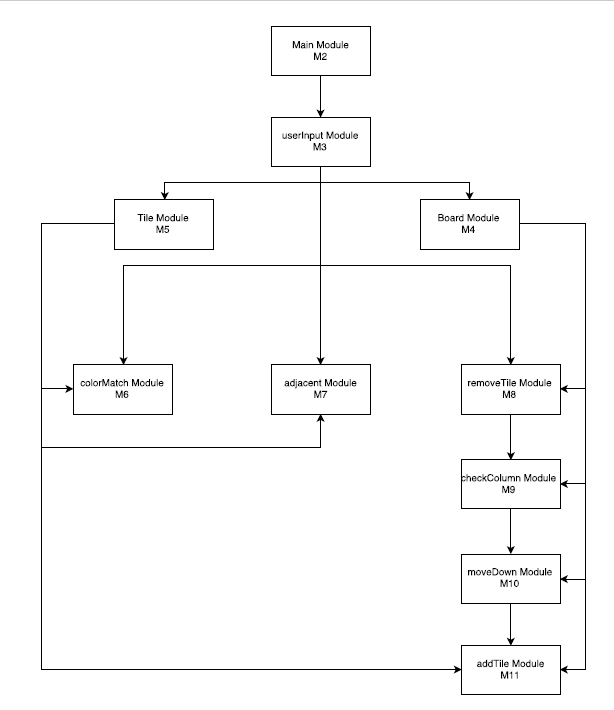
\includegraphics[width=17cm]{useTable}
\caption{Use Table}
\end{figure}
\newpage
\section{Schedule}
\subsection{Gantt Chart}

\begin{figure}[h!]
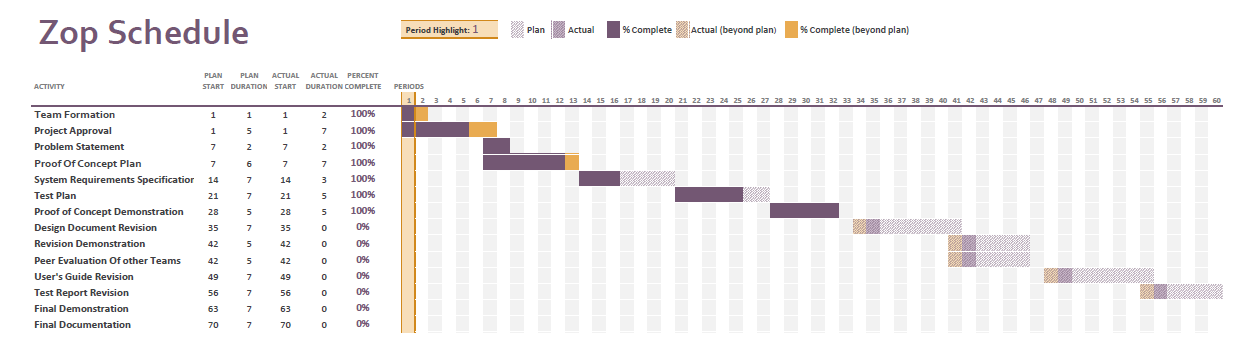
\includegraphics[width=17cm]{gantt}
\caption{Gantt Chart}
\end{figure}

\subsection{Pert Chart}

\begin{figure}[h!]
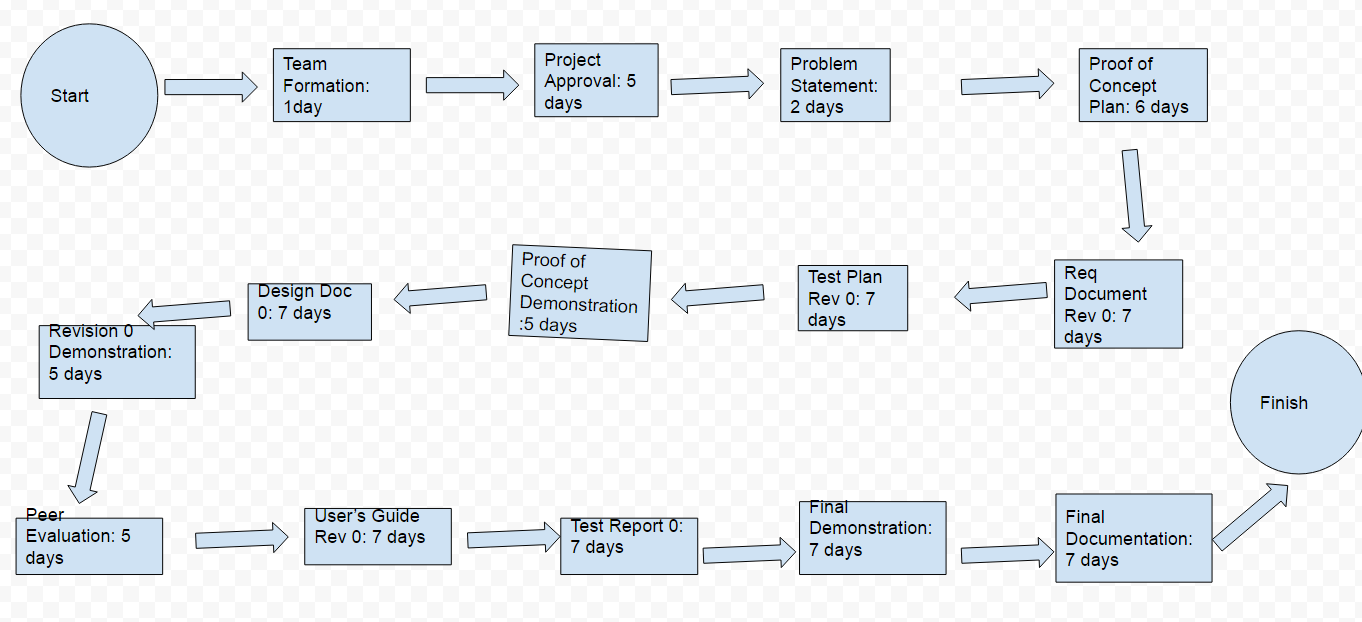
\includegraphics[width=17cm]{pert}
\caption{Pert Chart}
\end{figure}



\end{document}